% ====================================================================================

\begin{frame}
\frametitle{1969 - Special Interest Group on Computer Graphics and Interactive Techniques (SIGGRAPH)}

\begin{columns}

    % Image on the left
    \begin{column}{0.48\textwidth}
        \centering
        
\includegraphics[width=\linewidth]{assets/acmsig-logo.png}
    \end{column}

    % Text on the right
    \begin{column}{0.48\textwidth}
        In 1969, SIGGRAPH was officially established by the ACM after Sam Matsa and Andries van Dam highlighted the growing importance of Computer Graphics. The group had originated in 1963, with its founders giving talks at various conferences and short courses.
    \end{column}

\end{columns}

\end{frame}

% ====================================================================================

\begin{frame}
\frametitle{1969 - Graphical User Interface (GUI)}

\begin{columns}

    % Image on the left
    \begin{column}{0.48\textwidth}
        \centering
        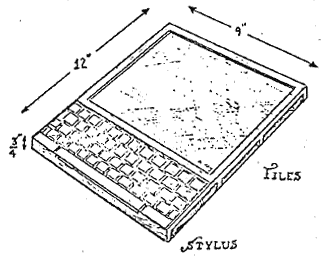
\includegraphics[width=\linewidth]{assets/Dynabook.png}
    \end{column}

    % Text on the right
    \begin{column}{0.48\textwidth}
        In 1969, Alan Kay started envisioning a  personal learning device for children, the "Dynabook". Recruited to work at Xerox PARC, he developed the idea of graphical representations of computing functions which led to the creation of  operating systems with a graphical user interface, or GUI.
    \end{column}

\end{columns}

\end{frame}

%====================================================================================

\begin{frame}
\frametitle{1969 - The First Framebuffer}

\begin{columns}

    % Image on the left
    \begin{column}{0.48\textwidth}
        \centering
        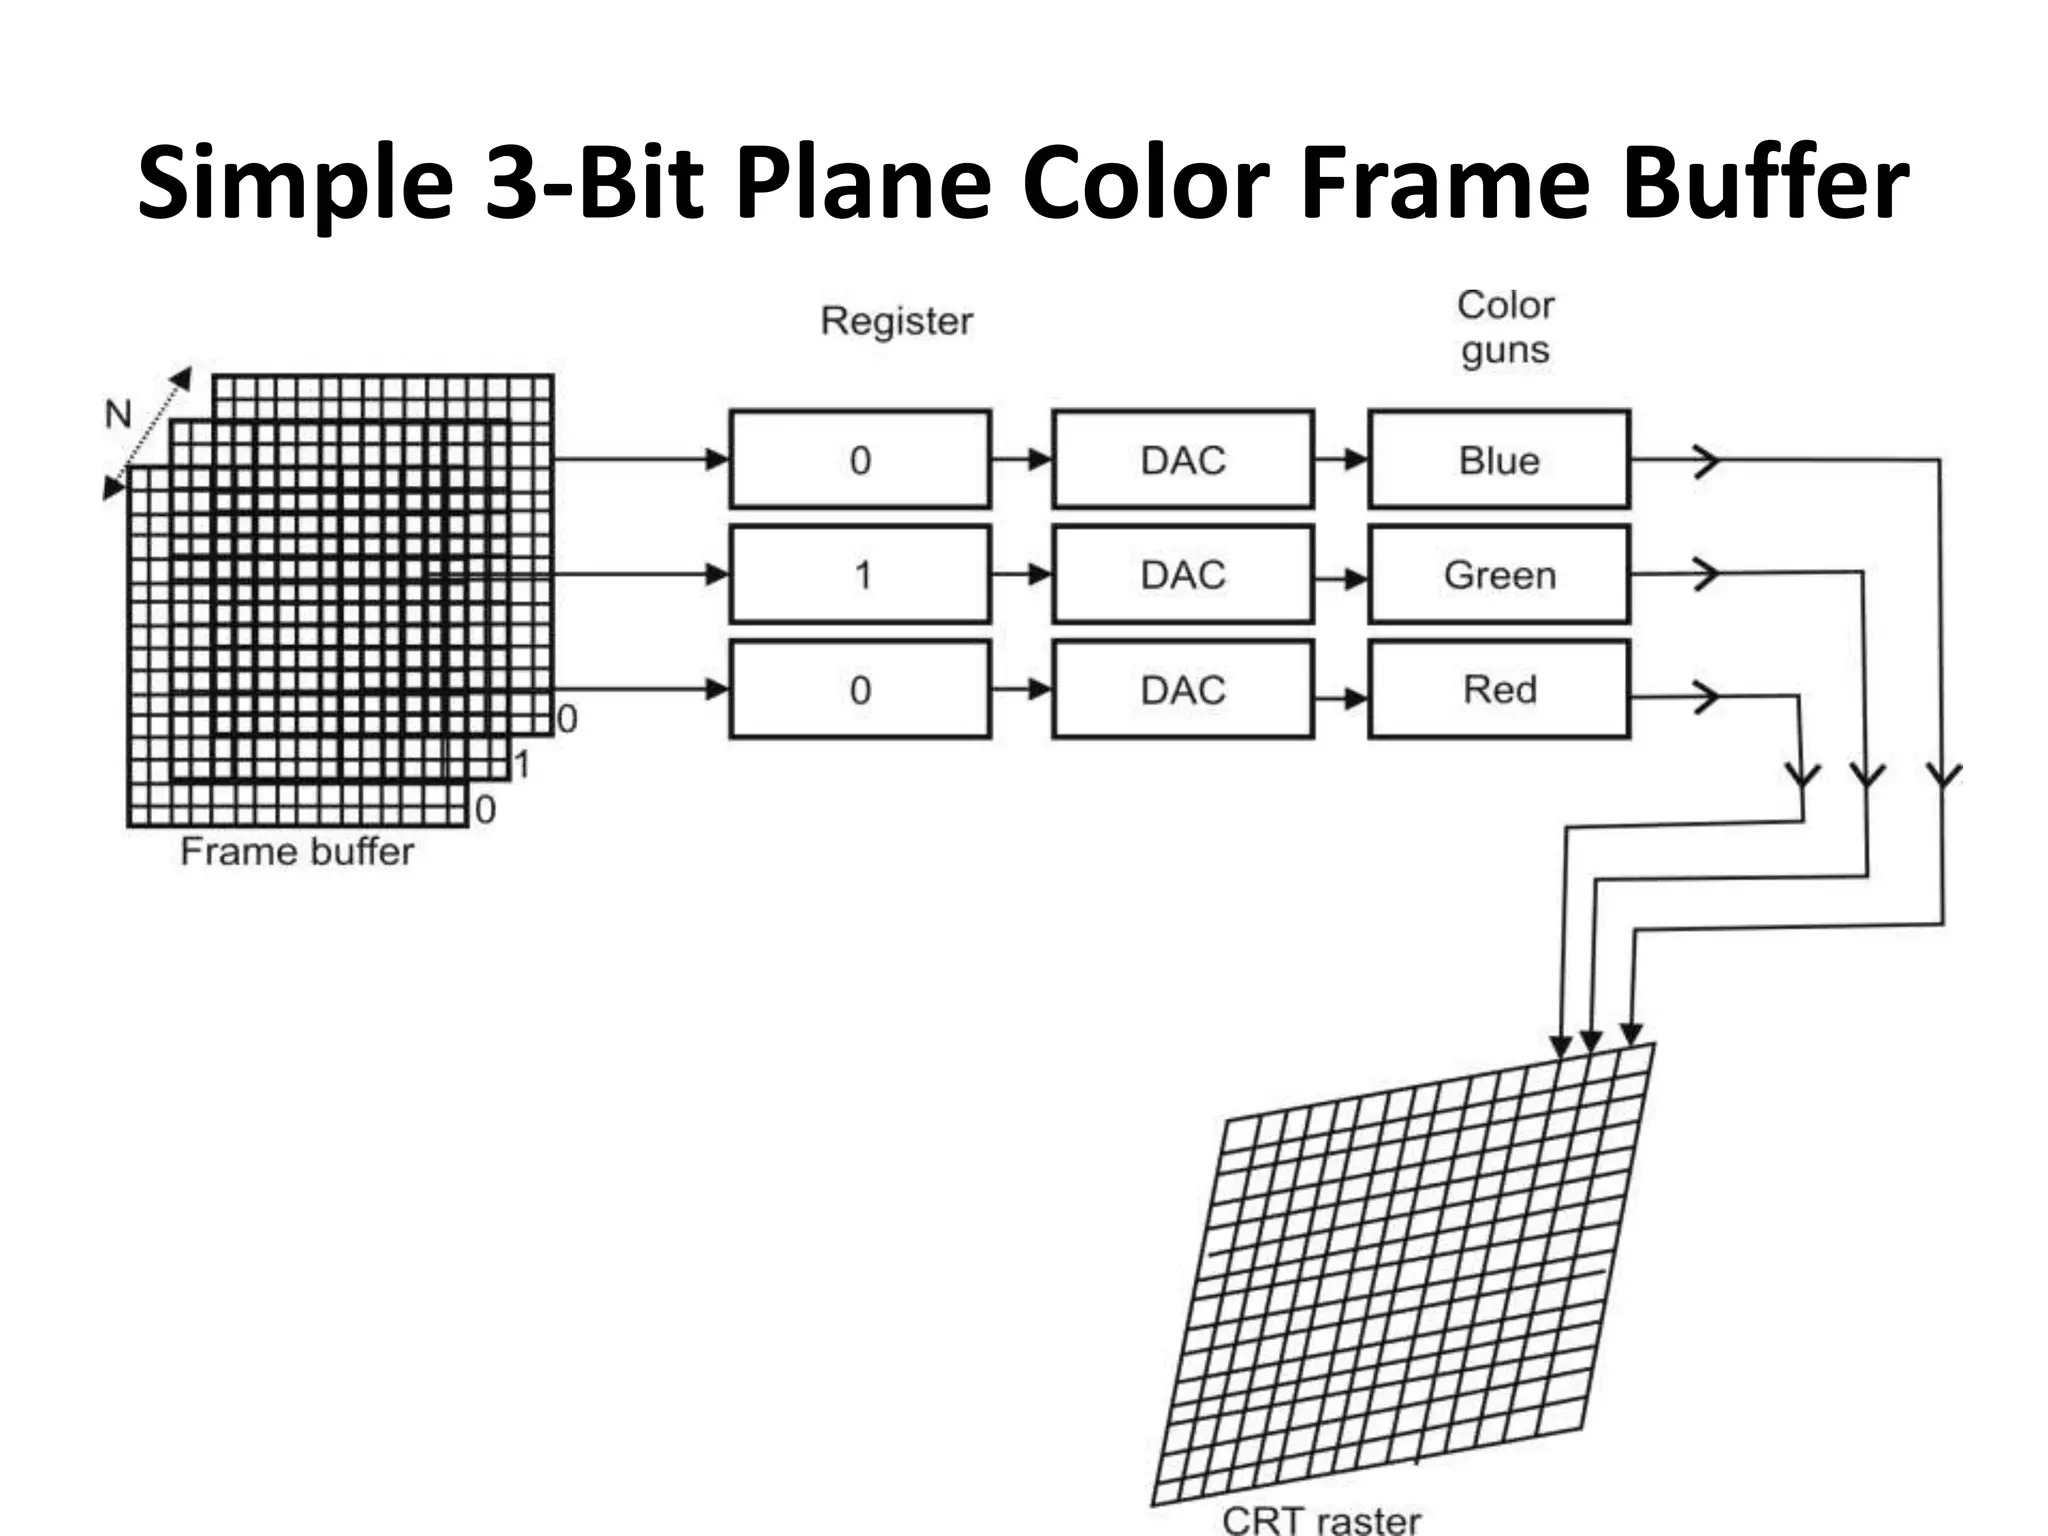
\includegraphics[width=\linewidth]{assets/3bitFramebuffer.jpg}
    \end{column}

    % Text on the right
    \begin{column}{0.48\textwidth}
        In 1969, the earliest functional frame buffer was a simple 3-bit paint program developed by Joan Miller at Bell Labs. Bell engineers developed several functional raster systems under the direction of A. Michael Noll, and by 1970 they had a system capable of producing real-time half-tone images on a raster display.

    \end{column}

\end{columns}

\end{frame}
